% ============================================================
% CHAPTER 9: SRE METHODOLOGY
% MCDA 5585 / 5586 Major Project Report
% Bhavik Kantilal Bhagat | A00494758 | Saint Mary's University
% ============================================================

\chapter{Methodologies}
\label{chap:methodologies}

During my co-op placement I adopted Site Reliability Engineering as the primary
methodology. I applied the four golden signals framework and SLI/SLO discipline
to address the observability gap exposed by the CAIS-Pricing Silent Outage and
the Meridian Incident. This chapter covers three areas: the SRE principles I
applied, the gap analysis that established the starting posture, and the
Dynatrace parity evaluation that framed the research question.


\FloatBarrier

\section{SRE Principles}
\label{sec:sre_principles}


Site Reliability Engineering is an operational discipline that applies
software engineering thinking to keeping production systems reliable at scale.
Its core concepts --- golden signals, Service Level Indicators (SLIs),
Service Level Objectives (SLOs), and error budgets --- provided the theoretical
backbone for every design decision I made during this co-op placement.

\subsection{The Four Golden Signals}

I discussed the four golden signals framework with Ms.\ Labos during a
dedicated knowledge-transfer session. These four signals define the minimum
instrumentation required to characterize service health:

\begin{enumerate}
    \item \textbf{Latency} --- \emph{How long does a request take?}
          For the IA platform, latency shows as Lambda function duration
          (P50, P95, P99 percentiles) and ECS service response time.
          Sustained P99 increases warn of resource saturation before
          errors appear.

    \item \textbf{Traffic} --- \emph{How much demand is on the system?}
          Measured as Lambda invocation count, SQS message ingestion rate,
          and MSK throughput (bytes in/out per second). Traffic anomalies
          often precede error and saturation signals.

    \item \textbf{Errors} --- \emph{What is the rate of failed requests?}
          Tracked as Lambda error and throttle counts, ECS task failures,
          and \texttt{NumberOfMessagesFailed} on SQS queues. An error rate
          crossing the defined threshold indicates a defect requiring
          immediate attention.

    \item \textbf{Saturation} --- \emph{How full is the service?}
          Saturation is the signal most relevant to the April~17,~2026
          Meridian incident. It is measured as Lambda concurrent
          execution count relative to the account concurrency limit,
          ECS task CPU and memory utilization, MSK consumer lag (the
          number of messages awaiting processing on a Kafka topic), and
          SQS queue depth with oldest-message age. A service approaching
          saturation degrades before it fails --- making this the most
          actionable of the four signals.
\end{enumerate}

Figure~\ref{fig:request_flow} illustrates how a request flows through
the monitored services, exposing each of the four golden signals at
different stages of the request lifecycle.

\begin{figure}[ht]
\centering
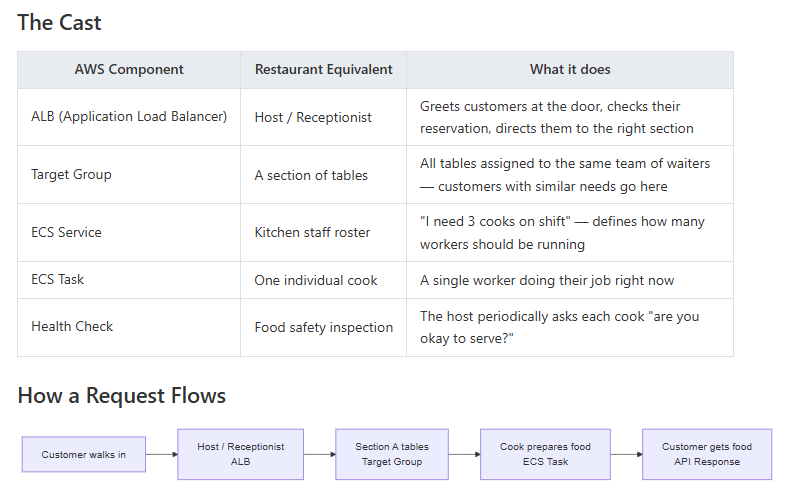
\includegraphics[width=0.90\textwidth]{figures/fig-request-flow-concepts.png}
\caption[Request Flow Through Monitored Services --- Golden Signals]{Request Flow Through Monitored Services --- Golden Signals at Each Stage}
\label{fig:request_flow}
\end{figure}

\subsection{Service Level Indicators and Objectives}

A \textbf{Service Level Indicator (SLI)} is the specific metric chosen
to represent one of the four golden signals for a service --- the
measurement. A \textbf{Service Level Objective (SLO)} is the target
threshold set on that measurement --- the acceptable limit.

For the IA platform, I selected the following SLIs and set corresponding
SLO thresholds, implemented as CloudWatch alarm trigger values:

\begin{itemize}
    \item \textbf{Lambda error rate}: SLI = \texttt{Errors / Invocations}
          per function. SLO threshold = fewer than 1\% of invocations
          result in an error over any 24-hour window. Implemented as a
          CloudWatch alarm with Metric Math expression
          \texttt{ErrorRate = Errors / Invocations}.

    \item \textbf{MSK consumer lag}: SLI = \texttt{EstimatedMaxTimeLag}
          per Meridian consumer group. SLO threshold = lag must remain
          below \textbf{10,000~messages} at any point. Derived from the
          April~17 post-mortem: lag reached 9~million messages before
          detection; a 10,000-message threshold would have fired within
          minutes of onset.

    \item \textbf{ECS CPU utilization}: SLI = task-level CPU utilization
          per cluster via Container Insights. SLO threshold = no service
          sustains above \textbf{80\%} over a 5-minute evaluation period.

    \item \textbf{SQS queue depth}: SLI = \texttt{ApproximateNumberOfMessagesVisible}
          per queue. SLO threshold = configurable per-queue maximum based
          on expected processing throughput.
\end{itemize}

These thresholds were encoded directly as CloudWatch alarm trigger
values --- each alarm fires when its SLI crosses the SLO boundary and
routes an SNS notification to the SRE team. This constitutes
\textbf{SLO-aligned alerting}: the alarms enforce the objectives but do
not compute running error budget consumption or burn rate.
This distinction is elaborated in the following subsection.

\subsection{Error Budgets}

An \textbf{error budget} is the complement of the SLO: the permitted
amount of unreliability before the objective is breached. For example,
if the Lambda error rate SLO is below 1\% over 24 hours, the error
budget is that 1\% of invocations permitted to fail.

During this co-op placement I did not implement automated error budget
tracking. The Grafana dashboard surfaces current SLI values and the
CloudWatch alarms fire at SLO breach --- which provides a reactive
signal that the budget has been consumed, but does not calculate how
quickly it is being drawn down. Full burn-rate alerting (requiring
Metric Math expressions dividing rolling error counts against the
rolling SLO budget) was identified as a post-placement enhancement.


\FloatBarrier

\section{Observability Gap Analysis}
\label{sec:observability_gap}


A prerequisite for building any monitoring platform is understanding the
current state of observability. Before I wrote a single line of code
for the centralized dashboard, I performed a structured gap analysis to characterize
what the IA platform could and could not see about itself.

\subsection{Pre-Co-op Placement Monitoring Posture}

At the commencement of my co-op placement in March~2026, the IA-SRE team's
monitoring posture exhibited the following deficiencies:

\begin{itemize}
    \item \textbf{No CloudWatch alarms on any Meridian service.} The
          Meridian Kafka-backed event pipeline --- the most
          business-critical component of the IA platform --- had zero
          proactive alerting. No alarms existed on MSK consumer lag,
          ECS task failure counts, Lambda error rates, or SQS queue
          depth for any Meridian-owned resource.

    \item \textbf{No centralized dashboard.} Monitoring was entirely
          fragmented. Operators who wished to check the health of a
          service were required to navigate to that service's individual
          CloudWatch console page. There was no eagle-eye view
          from which to assess the overall health of the platform.

    \item \textbf{Incomplete Container Insights coverage.} Of the six
          Meridian ECS clusters, only one (enabled in the DEV environment
          since July~2024) had Amazon CloudWatch Container Insights activated. The
          remaining five clusters were invisible to task-level CPU and
          memory telemetry.

    \item \textbf{No MSK consumer lag monitoring.} Despite Kafka
          consumer lag being the primary leading indicator of Meridian
          processing health --- as demonstrated conclusively by the
          Meridian Incident --- no metric or alarm existed for this
          signal. The \texttt{EstimatedMaxTimeLag} and
          \texttt{SumOffsetLag} metrics available natively from Amazon
          MSK were not surfaced anywhere.

    \item \textbf{No SLO tracking or error budget calculation.}
          The team had no defined SLIs, no published SLO targets, and
          therefore no basis for calculating error budgets or
          determining when the platform was in an unacceptable
          reliability state.

    \item \textbf{No automated resource inventory.} The inventory of
          Lambda functions, ECS clusters, and EC2 instances was
          maintained manually via Confluence pages and spreadsheets.
          This made it impossible to know, at any given moment, exactly
          which resources existed across all six platforms.

    \item \textbf{RPA bot monitoring limited to orchestrator UIs.}
          Blue Prism and UiPath bots were monitored exclusively through
          their respective orchestrator platforms (Blue Prism Orchestrator and
          UiPath Cloud). No CloudWatch integration existed, and there
          was no mechanism for the SRE team to receive proactive
          notification of bot failures or queue backlogs outside the
          orchestrator UI.

    \item \textbf{Reactive operational posture.} The cumulative effect
          of the above gaps was that the team's primary incident
          detection mechanism was business-team escalation. When a fund
          processing automation failed silently, the first signal
          received by the SRE team was a ticket or message from
          operations staff in Dublin, London, or Halifax who had noticed
          anomalous fund processing outputs. This reactive posture
          introduced structural latency between failure onset and
          engineering response.
\end{itemize}

\subsection{Gap Analysis Summary}

Table~\ref{tab:gap_analysis} summarizes the pre-placement gaps and the
post-placement resolutions for each monitoring domain.

\begin{tabularx}{\textwidth}{@{\hspace{\tabcolsep}}>{\raggedright\arraybackslash}p{0.18\textwidth}>{\raggedright\arraybackslash}X>{\raggedright\arraybackslash}X@{\hspace{\tabcolsep}}}
\caption[Observability Gap Analysis --- Pre- vs. Post-Co-op]{Observability Gap Analysis --- Pre- vs.\ Post-Co-op Placement} \label{tab:gap_analysis} \\
\hline
\rowcolor{smubrand}\textcolor{white}{\textbf{Domain}} & \textcolor{white}{\textbf{Pre-Co-op Placement State}} & \textcolor{white}{\textbf{Post-Co-op Placement State}} \\
\hline
\endfirsthead
\hline
\rowcolor{smubrand}\textcolor{white}{\textbf{Domain}} & \textcolor{white}{\textbf{Pre-Co-op Placement State}} & \textcolor{white}{\textbf{Post-Co-op Placement State}} \\
\hline
\endhead
\hline
\endfoot
\rowcolor{tablerowA} CloudWatch Alarms & 0 alarms on any IA resource & Dynamic alarms across AWS service categories \\
\rowcolor{tablerowB} Centralized Dashboard & None & CloudWatch, Grafana & Custom UI \\
\rowcolor{tablerowA} Container Insights & 1 of 6 Meridian clusters & 5 of 6 Meridian clusters \\
\rowcolor{tablerowB} MSK Consumer Lag & No monitoring & CloudWatch alarm on \texttt{EstimatedMaxTimeLag} ($<$30~sec detection) \\
\rowcolor{tablerowA} SLO Tracking & None & SLI/SLO targets defined; dashboard exposes current values \\
\rowcolor{tablerowB} Resource Inventory & Manual (Confluence) & Automated REST API (Lambda, ECS, EC2 across all platforms) \\
\rowcolor{tablerowA} Incident Detection & Business team escalation & Proactive alarm with SNS routing \\
\hline
\end{tabularx}


\FloatBarrier

\section{Dynatrace Parity Analysis}
\label{sec:dynatrace_parity}


A key question for this co-op placement is how closely an AWS-native observability stack can replicate
the capabilities of Dynatrace, and at what incremental cost. The PoC
investigation evaluated 25 Dynatrace features against five AWS tool
combinations to quantify achievable parity.

Table~\ref{tab:dynatrace_parity} summarizes the parity analysis for the
ten most operationally relevant Dynatrace capabilities to the IA platform.

\begin{tabularx}{\textwidth}{@{\hspace{\tabcolsep}}>{\raggedright\arraybackslash}p{0.32\textwidth}>{\centering\arraybackslash}p{0.08\textwidth}>{\centering\arraybackslash}p{0.08\textwidth}>{\centering\arraybackslash}p{0.08\textwidth}>{\centering\arraybackslash}p{0.16\textwidth}>{\centering\arraybackslash}p{0.08\textwidth}@{\hspace{\tabcolsep}}}
\caption[Dynatrace Capability Parity --- AWS-Native Stack vs Dynatrace]{Dynatrace Capability Parity --- AWS-Native Stack vs Dynatrace (selected features)} \label{tab:dynatrace_parity} \\
\hline
\rowcolor{smubrand}\textcolor{white}{\textbf{Dynatrace Feature}} & \textcolor{white}{\textbf{CW}} & \textcolor{white}{\textbf{+Grafana}} & \textcolor{white}{\textbf{+X-Ray}} & \textcolor{white}{\textbf{+App Signals}} & \textcolor{white}{\textbf{+Tempo}} \\
\hline
\endfirsthead
\hline
\rowcolor{smubrand}\textcolor{white}{\textbf{Dynatrace Feature}} & \textcolor{white}{\textbf{CW}} & \textcolor{white}{\textbf{+Grafana}} & \textcolor{white}{\textbf{+X-Ray}} & \textcolor{white}{\textbf{+App Signals}} & \textcolor{white}{\textbf{+Tempo}} \\
\hline
\endhead
\hline
\endfoot
\rowcolor{tablerowA} Alerting                  & \checkmark & \checkmark & --- & --- & --- \\
\rowcolor{tablerowB} Infrastructure Metrics    & \checkmark & \checkmark & --- & --- & --- \\
\rowcolor{tablerowA} Log Analytics             & \checkmark & \checkmark & --- & --- & --- \\
\rowcolor{tablerowB} Container Monitoring      & \checkmark & \checkmark & --- & \checkmark & --- \\
\rowcolor{tablerowA} Error Rate Tracking       & \checkmark & \checkmark & \checkmark & \checkmark & --- \\
\rowcolor{tablerowB} Latency Percentiles       & --- & \checkmark & \checkmark & \checkmark & \checkmark \\
\rowcolor{tablerowA} Distributed Trace Waterfall & --- & --- & \checkmark & --- & \checkmark \\
\rowcolor{tablerowB} Service Map / Topology    & --- & --- & \checkmark & \checkmark & --- \\
\rowcolor{tablerowA} SLO Management            & --- & --- & --- & \checkmark & --- \\
\rowcolor{tablerowB} Dependency Mapping        & --- & --- & \checkmark & \checkmark & --- \\
\rowcolor{tablerowA} \textbf{Parity (\% of 25 features)} & 30\% & 33\% & 60\% & 80\% & 83\% \\
\rowcolor{tablerowB} \textbf{Monthly Cost (est.)} & \$49 & \$68 & \$77 & \$232 & \$269 \\
\hline
\end{tabularx}

\noindent
Three capabilities remain \textbf{permanently outside the AWS-native reach}:
Davis~AI causal analysis (proprietary ML, no AWS equivalent); automatic
baselining (Dynatrace learns per-service baselines over weeks; AWS alarms
require manual thresholds); and session replay (full DOM capture, not
available in any OSS tool). These account for approximately 9--10\% of
the functional gap that no combination of AWS tools can close.

\paragraph{Adopted stack.}
The PoC I delivered in this co-op placement corresponds to the
\textbf{CloudWatch + Grafana + X-Ray} column: 60\% parity at approximately
\$77/month. Application Signals (the path to 80\% parity) requires deploying
an ADOT sidecar on each ECS service and is scoped as post-placement work.
The gap-to-tooling mapping contextualizes what the PoC does and does not cover throughout the Implementation chapter. This methodological foundation---combining golden signals, gap analysis, and parity assessment---established the engineering rationale for every implementation decision.

% Keep all floats within this chapter
\FloatBarrier